%% Лабораторная работа № 1 по курсу «Информационный поиск».
%% Оформление соответствует TeX-шаблону report_pattern преподавателя.

\documentclass[pdf,unicode,12pt,a4paper,oneside,fleqn]{article}

\usepackage{styles/log-style}

\begin{document}

\begin{titlepage}
\begin{center}
\bfseries

{\Large Московский авиационный институт\\
(национальный исследовательский университет)}

\vspace{48pt}

{\large Институт № 8 «Компьютерные науки»}

\vspace{72pt}

Лабораторная работа \textnumero 1 по курсу
\enquote{Информационный поиск}

\vspace{18pt}

{\large \enquote{Добыча корпуса документов}}

\end{center}

\vspace{72pt}

\begin{flushright}
\begin{tabular}{rl}
Студент: & Д.\,А. Кулешов \\
Преподаватель: & А.\,А. Кухтичев \\
Группа: & М8О-408Б-23 \\
Отметка о сдаче: & \rule{35mm}{0.4pt} \\
Оценка: & \rule{35mm}{0.4pt} \\
\end{tabular}
\end{flushright}

\vfill

\begin{center}
\bfseries
Москва, 2026
\end{center}
\end{titlepage}

\pagebreak

\CWHeader{Лабораторная работа \textnumero 1
\enquote{Добыча корпуса документов}}

\section{Задание}

Цель работы --- выбрать источники для будущего поискового индекса, получить
примеры документов, изучить их формат и метаданные, выделить основной текст и
оценить количественные характеристики выбранного корпуса.

В соответствии с заданием необходимо:

\begin{itemize}
    \item использовать не менее двух источников документов;
    \item скачать примеры документов и указать источники данных;
    \item изучить состав сырого документа, его разметку и метаданные;
    \item выделить из сырого представления основной текст;
    \item найти существующие поисковые системы, работающие с выбранными
    источниками;
    \item выполнить несколько запросов и указать недостатки полученной выдачи;
    \item определить количество документов, общий и средний размер сырых
    документов, общий и средний размер выделенного текста.
\end{itemize}

В качестве предметной области я выбрал англоязычные технические тексты по
компьютерным наукам и информационным технологиям. В корпус входят три источника:
Wikipedia, arXiv HTML и Microsoft Learn. Wikipedia содержит энциклопедические
статьи, arXiv --- научные публикации, Microsoft Learn --- прикладную техническую
документацию. Таким образом, документы относятся к общей технической тематике,
но отличаются жанром и структурой.

\section{Краткое описание метода решения}

Анализ каждого источника выполняется в отдельном Jupyter Notebook. Для получения
документов используются официальные способы обнаружения данных: MediaWiki API,
Atom API arXiv и sitemap Microsoft Learn. После загрузки я изучаю структуру
сырого документа и метаданные, выделяю основной текст по правилам конкретного
источника, измеряю размеры и вручную проверяю несколько страниц.

Для работы используются Python, \texttt{requests}, Beautiful Soup,
\texttt{lxml}, \texttt{pandas} и \texttt{matplotlib}. Зависимости фиксируются
проектом и устанавливаются через \texttt{uv}. Воспроизводимый запуск анализа
выполняется командами:

\begin{lstlisting}[language=bash]
uv sync
uv run jupyter notebook notebooks
\end{lstlisting}

В Jupyter необходимо последовательно выполнить \texttt{Run All} для файлов
\texttt{wikipedia.ipynb}, \texttt{arxiv.ipynb} и
\texttt{microsoft\_learn.ipynb}. Все строки и файлы обрабатываются в UTF-8.

\section{Журнал выполнения задания}

\subsection{Подготовка и порядок анализа}

Для каждого источника я использовал одинаковую последовательность действий:

\begin{enumerate}
    \item обнаружил адреса документов с помощью официального API или sitemap;
    \item загрузил 30 примеров и сохранил их локально;
    \item определил поля метаданных и область страницы с основным содержимым;
    \item удалил служебные блоки и нормализовал пробельные символы;
    \item измерил размер сырого представления и выделенного текста в байтах UTF-8;
    \item подсчитал слова разделением текста по пробельным символам;
    \item проверил существующий поиск и записал наблюдаемые ограничения.
\end{enumerate}

Локальный кэш размещается в \texttt{notebooks/samples}. Он исключён из Git, так
как содержит загруженные документы, но позволяет повторно выполнять анализ без
новых запросов к внешним сайтам. Код и результаты анализа сохраняются
непосредственно в ноутбуках.

Размер сырого документа вычисляется как длина его сохранённого представления в
байтах UTF-8. Размер текста вычисляется после выделения основного содержимого и
нормализации пробелов. Среднее значение равно сумме размеров, делённой на число
документов. Для сравнения источников также рассчитана доля текста в сыром
документе.

\subsection{Wikipedia}

Для Wikipedia использован официальный MediaWiki API:

\begin{center}
\url{https://en.wikipedia.org/w/api.php}
\end{center}

В выборку включены страницы из категорий \texttt{Computer science},
\texttt{Engineering}, \texttt{Mathematics}, \texttt{Physics},
\texttt{Chemistry} и \texttt{Biology}. Сначала методом
\texttt{categorymembers} получаются кандидаты, затем для каждой страницы
запрашиваются идентификатор, заголовок, URL, Wikidata ID и поле
\texttt{extract}.

Основные параметры запроса выглядят следующим образом:

\begin{lstlisting}[language=Python]
response = session.get(API_URL, params={
    'action': 'query',
    'format': 'json',
    'formatversion': 2,
    'pageids': page_id,
    'prop': 'extracts|info|pageprops',
    'explaintext': 1,
    'inprop': 'url',
}, timeout=60)
\end{lstlisting}

Параметр \texttt{explaintext=1} просит MediaWiki вернуть обычный текст без
HTML-разметки. Поэтому выделение текста для этого источника состоит в чтении
поля \texttt{extract} и схлопывании повторных пробельных символов:

\begin{lstlisting}[language=Python]
text = re.sub(r'\s+', ' ', page.get('extract', '')).strip()
\end{lstlisting}

Сырой документ в этом ноутбуке --- JSON-объект API, а не HTML страницы. В нём
сохраняются \texttt{pageid}, \texttt{title}, \texttt{fullurl},
\texttt{wikibase\_item}, категория выборки и текстовый \texttt{extract}. Это
важно учитывать при сравнении размеров: доля текста в JSON Wikipedia ожидаемо
выше, чем доля текста в HTML двух других источников.

В качестве ручного примера проверена статья
\href{https://en.wikipedia.org/wiki/Computer_science}{Computer science}. Её
\texttt{pageid} равен 5323, размер JSON в выборке --- 30 814 байт, размер
выделенного текста --- 30 137 байт, число слов --- 4 306. Заголовок, URL и
Wikidata ID были получены отдельно от текста и не потерялись при нормализации.

Результат анализа Wikipedia: все 30 документов содержат непустой связный текст.
Общий размер JSON-документов составил 643 895 байт, выделенного текста ---
623 248 байт. Средний документ содержит 3 121,37 слова. Разница между сырьём и
текстом небольшая, потому что MediaWiki API уже выполнил удаление HTML-разметки.
Источник подходит для корпуса, но при массовой загрузке HTML правила выделения
текста придётся проверять отдельно.

\subsection{arXiv HTML}

Метаданные arXiv получены через Atom API:

\begin{center}
\url{https://export.arxiv.org/api/query}
\end{center}

Для анализа выбраны по 10 публикаций из категорий \texttt{cs.IR},
\texttt{cs.AI} и \texttt{cs.CL}. Таким образом, выборка состоит из 30
документов и охватывает информационный поиск, искусственный интеллект и
компьютерную лингвистику. Из Atom сохраняются идентификатор статьи, название,
авторы, аннотация, категории, даты публикации и обновления, лицензия.

Сырой документ загружается с адреса
\texttt{https://arxiv.org/html/<arxiv-id>}. Между HTML-запросами установлена
пауза в одну секунду. При кодах 429 и 503 запрос повторяется после увеличенной
паузы либо значения заголовка \texttt{Retry-After}.

Основное содержимое находится в \texttt{article.ltx\_document},
\texttt{article} или \texttt{main}. После выбора корневого узла удаляются
скрипты, стили, навигация, боковые панели и подвал. Текст собирается из
заголовков, абзацев, элементов списков и блоков кода:

\begin{lstlisting}[language=Python]
article = soup.select_one('article.ltx_document, article, main')
for node in article.select('script, style, nav, aside, footer'):
    node.decompose()
blocks = [
    node.get_text(' ', strip=True)
    for node in article.select('h1, h2, h3, p, li, pre')
]
text = re.sub(r'\s+', ' ', ' '.join(blocks)).strip()
\end{lstlisting}

HTML arXiv создаётся из LaTeX и содержит большое количество классов, формул и
служебной разметки. Формулы переходят в линейное текстовое представление, поэтому
часть двумерной структуры теряется. Это ограничение допустимо для полнотекстового
поиска, но исходный HTML необходимо сохранять, чтобы в дальнейшем можно было
улучшить правила обработки.

В качестве примера вручную разобрана статья
\href{https://arxiv.org/html/2610.28435v1}{Multimodal Reranking Is a System One
Decision}. Её HTML занимает 393 967 байт, выделенный текст --- 36 089 байт,
число слов --- 5 806. В текст попали название, разделы и абзацы статьи, а
навигация и оформление страницы были удалены.

Результат анализа arXiv: получено 30 непустых HTML-статей. Их общий сырой размер
равен 16 108 664 байтам, а размер выделенного текста --- 2 242 943 байтам.
Средняя статья содержит 11 931,97 слова. Это самый длинный и самый сложный по
разметке источник. Он даёт точную научную терминологию, но требует аккуратной
обработки формул, библиографии и LaTeXML-разметки.

\subsection{Microsoft Learn}

Адреса страниц Microsoft Learn получены через индекс sitemap:

\begin{center}
\url{https://learn.microsoft.com/_sitemaps/sitemapindex.xml}
\end{center}

Из sitemap выбираются только англоязычные адреса \texttt{/en-us/}. Исключаются
ответы пользователей, видео, события, профили, страницы сертификатов,
API-справочник и архив старых версий. Чтобы не получить 30 однотипных страниц
одного продукта, документы поочерёдно выбираются из разделов Azure, SQL,
Windows, Linux, Security, Power BI, DevOps, Cosmos DB, Semantic Kernel, C++,
Defender и AI.

Основной материал страницы находится внутри \texttt{main}. Из него удаляются
скрипты, стили, навигация, кнопки, уведомления, метаданные статьи, оглавление и
форма обратной связи. Код и таблицы сохраняются, так как для технической
документации они содержат значимые термины.

\begin{lstlisting}[language=Python]
main = soup.select_one('main')
for node in main.select(
    'script, style, nav, aside, footer, button, .notification, '
    '#article-header, #article-metadata, '
    '#site-user-feedback-footer, .doc-outline'
):
    node.decompose()

blocks = [
    node.get_text(' ', strip=True)
    for node in main.select('h1, h2, h3, p, li, pre, table')
]
\end{lstlisting}

Из метатегов отдельно сохраняются \texttt{document\_id}, описание, автор и
дата. Из элемента \texttt{link rel="canonical"} извлекается канонический URL.
Такое разделение позволяет сохранить метаданные для будущей фильтрации, но не
добавлять их повторно в основной текст.

В качестве ручного примера проверена страница
\href{https://learn.microsoft.com/en-us/cosmos-db/index-vector-data}{Index
vector data in Cosmos DB}. Её HTML занимает 61 456 байт, выделенный текст ---
14 273 байта, число слов --- 2 149. После очистки остались описание векторного
индекса, параметры, списки, таблицы и примеры конфигурации.

Результат анализа Microsoft Learn: получено 30 документов из разных продуктовых
разделов. Общий HTML занимает 1 770 272 байта, выделенный текст --- 307 385 байт,
среднее число слов равно 1 474,33. Основной текст заметно короче, чем у arXiv,
однако в нём встречаются важные для поиска имена команд, классов, параметров и
фрагменты кода. Удаление навигации и повторяющихся служебных блоков обязательно.

\subsection{Сопоставление результатов анализа метаданных}

Состав сохранённых метаданных приведён в таблице~\ref{tab:metadata}.

\begin{table}[htbp]
\centering
\caption{Метаданные исследованных источников}
\label{tab:metadata}
\begin{tabular}{|p{0.18\textwidth}|p{0.36\textwidth}|p{0.36\textwidth}|}
\hline
\textbf{Источник} & \textbf{Основные поля} & \textbf{Назначение} \\
\hline
Wikipedia & \texttt{pageid}, заголовок, URL, Wikidata ID, категория &
идентификация статьи и связь с категорией \\
\hline
arXiv & arXiv ID, авторы, категории, даты, лицензия, аннотация &
поиск научных работ и фильтрация по предметной области \\
\hline
Microsoft Learn & document ID, продукт, автор, дата, описание, canonical URL &
идентификация версии документа и принадлежности продукту \\
\hline
\end{tabular}
\end{table}

Анализ показал, что во всех трёх источниках можно сохранить устойчивый
идентификатор, заголовок и URL. Дополнительные поля различаются: Wikipedia даёт
связь с Wikidata, arXiv --- авторов, предметные категории и лицензию, Microsoft
Learn --- продукт, автора документа и дату. Эти поля не следует смешивать с
основным текстом, но их нужно сохранить для фильтрации и будущего зонного поиска.

\subsection{Возникшие проблемы и выбранные решения}

Для каждого источника был создан отдельный ноутбук. Это упростило повторный
запуск и позволило не смешивать разные правила получения и очистки документов.

При работе с Wikipedia выяснилось, что полный \texttt{extract} удобнее получать
по одной странице. Сначала я загружаю небольшой список кандидатов из нескольких
категорий, а затем последовательно запрашиваю содержимое. Пустые и слишком
короткие статьи не включаются: минимальный объём установлен равным 200 словам.

Для arXiv основной проблемой стала стоимость повторной загрузки больших
HTML-страниц и возможность временных ответов 429 или 503. Поэтому запросы
выполняются последовательно, между ними есть пауза, а готовая выборка кэшируется.
В выборку включаются только статьи, для которых доступна HTML-версия. Это создаёт
некоторое смещение выборки, поскольку не все документы arXiv имеют HTML.

У Microsoft Learn один sitemap может содержать много однотипных страниц одного
раздела. Простое чтение первых 30 адресов дало бы нерепрезентативную выборку.
Поэтому я разделил адреса по продуктам и выбирал их поочерёдно. Дополнительно
исключил страницы API и старых версий. После очистки проверяется минимальный объём
в 250 слов.

Единый CSS-селектор для всех трёх источников использовать нельзя. Wikipedia в
ноутбуке уже возвращает текст в JSON, arXiv хранит статью в \texttt{article}, а
Microsoft Learn --- в \texttt{main}. Я оставил отдельные функции выделения
текста. Это немного увеличивает код, но делает правила понятными и не приводит к
смешиванию основного содержимого с навигацией.

Размеры источников сначала выглядели несопоставимыми. Причина состоит в том, что
у Wikipedia сырой документ --- компактный JSON с уже очищенным
\texttt{extract}, а у arXiv и Microsoft Learn --- полный HTML. Поэтому в
результатах я указываю не только абсолютные размеры, но и явно определяю, что
именно считается сырым документом.

\section{План тестирования}

План составлен так, чтобы проверить загрузку, повторяемость, качество выделения
текста и корректность статистики. Тесты выполняются отдельно для каждого
ноутбука. План приведён в таблице~\ref{tab:tests}.

\normalsize
\begin{longtable}{|>{\centering\arraybackslash}p{0.05\textwidth}|p{0.25\textwidth}|p{0.42\textwidth}|p{0.15\textwidth}|}
\caption{План и результаты тестирования}\label{tab:tests}\\
\hline
\textbf{№} & \textbf{Проверка} & \textbf{Ожидаемый результат} &
\textbf{Результат} \\
\hline
\endfirsthead
\multicolumn{4}{r}{Продолжение таблицы~\thetable}\\
\hline
\textbf{№} & \textbf{Проверка} & \textbf{Ожидаемый результат} &
\textbf{Результат} \\
\hline
\endhead
1 & Установка через \texttt{uv sync} & Все зависимости устанавливаются без
ручного подбора версий & Пройдено \\
\hline
2 & Выполнение \texttt{Run All} & Ячейки выполняются последовательно,
статистика выводится & Пройдено \\
\hline
3 & Число документов & В каждом источнике получено ровно 30 документов &
Пройдено \\
\hline
4 & Уникальность идентификаторов & Внутри выборки нет повторяющихся page ID,
arXiv ID и URL & Пройдено \\
\hline
5 & Наличие текста & После очистки нет пустых документов & Пройдено \\
\hline
6 & Порог длины & Wikipedia содержит не менее 200 слов, Learn --- не менее
250 слов & Пройдено \\
\hline
7 & Метаданные & У документов есть идентификатор, заголовок и URL & Пройдено \\
\hline
8 & Размеры & Суммы размеров совпадают с суммой строк таблицы документов &
Пройдено \\
\hline
9 & Ручная проверка текста & Для одной страницы каждого источника отсутствуют
меню и служебные блоки & Пройдено \\
\hline
10 & Повторный запуск & При наличии кэша используются те же документы без
повторной загрузки & Пройдено \\
\hline
11 & Существующий поиск & Ссылки на поиск открываются и возвращают результаты &
Пройдено \\
\hline
\end{longtable}
\normalsize

Проверка уникальности выполняется до добавления документа в выборку. В
Wikipedia используется множество \texttt{seen\_page\_ids}, в arXiv ---
\texttt{seen\_ids}, в Microsoft Learn --- \texttt{seen\_urls}. Поэтому одна и
та же страница не учитывается два раза в статистике.

Ручная проверка проводилась сравнением страницы в браузере с полем \texttt{text}
в таблице ноутбука. Для Wikipedia проверена статья \texttt{Computer science},
для arXiv --- \texttt{2610.28435v1}, для Microsoft Learn --- страница об
индексации векторов в Cosmos DB.

В этой работе не создаётся самостоятельная поисковая программа или интерфейс
ввода запросов: результатом является воспроизводимый анализ источников в трёх
ноутбуках. Поэтому требование о консольной утилите для поисковых лабораторных к
данному этапу не применяется. Результаты каждого теста остаются в выходных
ячейках ноутбуков.

\pagebreak

\section{Результаты}

\subsection{Количественные характеристики}

Результаты измерений приведены в таблице~\ref{tab:statistics}. Размеры указаны в
байтах UTF-8.

\begin{table}[htbp]
\centering
\small
\caption{Размеры документов исследовательской выборки}
\label{tab:statistics}
\begin{tabular}{|p{0.29\textwidth}|r|r|r|r|}
\hline
\textbf{Показатель} & \textbf{Wikipedia} & \textbf{arXiv} &
\textbf{Microsoft Learn} & \textbf{Всего} \\
\hline
Количество документов, шт. & 30 & 30 & 30 & \textbf{90} \\
\hline
Сырой размер, байт & 643 895 & 16 108 664 & 1 770 272 &
\textbf{18 522 831} \\
\hline
Размер текста, байт & 623 248 & 2 242 943 & 307 385 &
\textbf{3 173 576} \\
\hline
Средний сырой размер, байт/док. & 21 463,17 & 536 955,47 & 59 009,07 &
\textbf{205 809,23} \\
\hline
Средний размер текста, байт/док. & 20 774,93 & 74 764,77 & 10 246,17 &
\textbf{35 261,96} \\
\hline
\end{tabular}
\end{table}

Среднее количество слов в документе равно 3 121,37 для Wikipedia, 11 931,97 для
arXiv и 1 474,33 для Microsoft Learn. Наиболее длинными оказались научные статьи
arXiv. Документация Microsoft Learn в среднем короче, но содержит больше кода,
таблиц и узких названий параметров.

Доля выделенного текста в сыром представлении составляет 96,79 \% для
Wikipedia, 13,92 \% для arXiv и 17,36 \% для Microsoft Learn. Для всей выборки
она равна 17,13 \%. Высокое значение Wikipedia связано не с отсутствием
служебных элементов на веб-странице, а с тем, что в данной лабораторной сырьём
считается JSON API с уже подготовленным текстовым \texttt{extract}.

Полученные 90 документов являются исследовательской выборкой для проверки
источников и правил выделения текста. Они не являются полным корпусом. Для
дальнейших лабораторных массовый сбор должен выполняться поисковым роботом, а
обработка --- потоково, без загрузки всего корпуса в оперативную память.

\begin{figure}[htbp]
\centering
\begin{minipage}{0.48\textwidth}
    \centering
    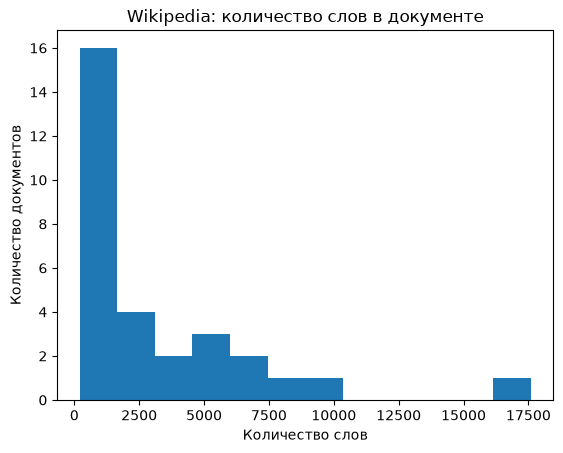
\includegraphics[width=\linewidth]{../images/wikipedia_document_lengths.png}
\end{minipage}
\hfill
\begin{minipage}{0.48\textwidth}
    \centering
    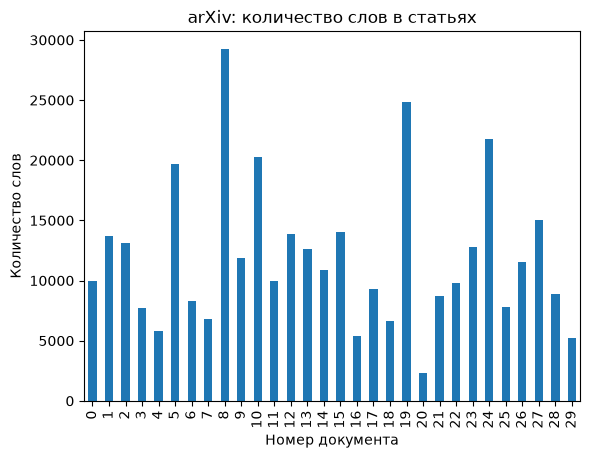
\includegraphics[width=\linewidth]{../images/arxiv_document_lengths.png}
\end{minipage}

\vspace{6mm}

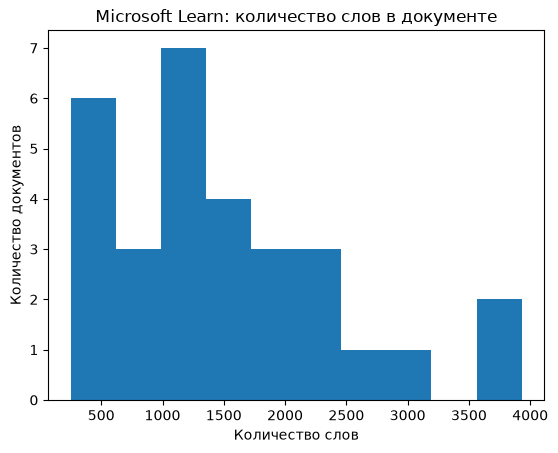
\includegraphics[width=0.55\textwidth]{../images/microsoft_learn_document_lengths.png}
\caption{Распределение числа слов в исследованных документах}
\label{fig:lengths}
\end{figure}

Графики построены непосредственно в ноутбуках по полю \texttt{word\_count}.
Они подтверждают различие источников: arXiv содержит наиболее длинные статьи и
большой разброс объёма, Wikipedia сочетает средние статьи с отдельными длинными
обзорными и справочными страницами, а документы Microsoft Learn в среднем
короче. Поэтому один общий порог размера для всех источников привёл бы к
неравномерному отбору документов.

\subsection{Проверка существующего поиска}

Согласно условию задания, корпус можно использовать только при наличии уже
существующего поиска. Для всех трёх источников такой поиск есть. Результаты
проверки приведены в таблице~\ref{tab:search}.

\begin{table}[htbp]
\centering
\small
\caption{Проверка существующих поисковых систем}
\label{tab:search}
\begin{tabular}{|p{0.14\textwidth}|p{0.21\textwidth}|p{0.23\textwidth}|p{0.27\textwidth}|}
\hline
\textbf{Источник} & \textbf{Запрос} & \textbf{Наблюдение} &
\textbf{Недостаток} \\
\hline
Wikipedia & neural information retrieval & находятся статьи по отдельным понятиям &
нет научных публикаций и документации в той же выдаче \\
\hline
Wikipedia & python memory model & есть результаты о Python и памяти &
узкий практический вопрос плохо соответствует названиям статей \\
\hline
arXiv & neural information retrieval & находятся профильные научные работы &
нет справочных и прикладных материалов \\
\hline
arXiv & vector database & есть работы о векторном поиске & часть результатов
тематически близка, но не отвечает на практический вопрос \\
\hline
Microsoft Learn & site:learn.\newline microsoft.com vector search HNSW & находится
документация по векторным индексам & смешиваются страницы разных продуктов и
версий \\
\hline
Microsoft Learn & site:learn.\newline microsoft.com python async memory & находятся
материалы по Python и асинхронности & неоднозначные слова относятся к нескольким
продуктам \\
\hline
\end{tabular}
\end{table}

Проверялись следующие поисковые интерфейсы:

\begin{itemize}
    \item \href{https://en.wikipedia.org/w/index.php?search=neural+information+retrieval}{поиск Wikipedia};
    \item \href{https://arxiv.org/search/?query=\%22neural+information+retrieval\%22\&searchtype=all}{поиск arXiv};
    \item \href{https://www.google.com/search?q=site:learn.microsoft.com+vector+search+HNSW}{Google с ограничением Microsoft Learn}.
\end{itemize}

Основной общий недостаток состоит в разделении источников. Пользователь не может
одним запросом одновременно получить энциклопедическое объяснение, научные
статьи и практическую документацию. Это обосновывает создание собственного
индекса по объединённому корпусу.

\subsection{Выполнение требований задания}

По результатам анализа выполнены все пункты задания первой лабораторной работы:

\begin{itemize}
    \item использованы три источника при требуемых двух;
    \item получены локальные примеры и указаны способы их загрузки;
    \item описаны сырой формат, разметка и метаданные каждого источника;
    \item выделен основной текст и вручную проверены три конкретные страницы;
    \item рассчитаны количество документов, общий и средний размер сырья и текста;
    \item проверены существующие поисковые системы и разобраны шесть запросов;
    \item зафиксированы ограничения выборки и способов выделения текста.
\end{itemize}

Метрики P, DCG, NDCG и ERR здесь не вычисляются, поскольку в первой лабораторной
не строится собственная ранжированная выдача и нет набора экспертных оценок
релевантности. Вместо этого, как требует задание lesson-01, существующий поиск
оценивается качественно по конкретным запросам. Количественная оценка
ранжирования должна выполняться в отдельной лабораторной после реализации
поиска.

Выборка из 90 документов нужна именно для анализа форматов. Она не заменяет
полный входной корпус. Общий README курса требует не менее 30 000 документов, а
для применения решения на оценку «отлично» --- больше одного миллиона
документов, не помещающихся целиком в оперативную память. Поэтому масштаб
полного корпуса проверяется отдельно при массовом обходе источников; в этом
отчёте он не подменяется размером исследовательской выборки.

\subsection{Пригодность корпуса для следующих работ}

Выбранные источники подходят для дальнейшей разработки поисковой системы по
следующим причинам:

\begin{itemize}
    \item у каждого документа есть устойчивый идентификатор и канонический URL;
    \item доступны способы массового обнаружения документов: категории
    MediaWiki, Atom API arXiv и sitemap Microsoft Learn;
    \item основной текст можно отделить от служебных блоков;
    \item документы содержат естественный язык, технические термины, код и формулы;
    \item источники имеют существующий поиск для последующего сравнения;
    \item разные жанры позволяют проверять поиск не только на одном типе текста.
\end{itemize}

При массовом сборе необходимо сохранить сырой документ вместе с метаданными и
хешем содержимого. Тогда правила выделения текста можно менять без повторного
скачивания страниц. Для исключения дублей достаточно установить уникальность
пары «источник --- идентификатор документа». Сами 30 документов на источник
нужны для анализа, а не для ограничения размера будущего корпуса.

\section{Выводы}

В работе я исследовал три источника англоязычных технических документов:
Wikipedia, arXiv HTML и Microsoft Learn. Для каждого источника были загружены 30
примеров, изучены формат сырого документа и метаданные, реализовано выделение
основного текста и рассчитана статистика.

Суммарный объём 90 сырых документов составил 18 522 831 байт, а объём
выделенного текста --- 3 173 576 байт. Наибольший средний объём текста получен у
arXiv --- 74 764,77 байта и 11 931,97 слова на документ. Wikipedia в выбранном
API-представлении содержит минимальную долю служебных данных. Microsoft Learn
даёт наиболее короткие документы, но содержит полезные команды, таблицы и
названия программных компонентов.

Единого правила выделения текста оказалось недостаточно. Для Wikipedia текст
берётся из API-поля \texttt{extract}, для arXiv выбирается узел
\texttt{article}, для Microsoft Learn --- \texttt{main} с дополнительным
удалением служебных блоков. Отдельные правила проще проверять и изменять при
обновлении разметки сайтов.

Существующий поиск доступен для всех источников, поэтому условие задания
выполнено. При этом ни одна из проверенных систем не объединяет все три вида
документов. Собственная поисковая система сможет применять одинаковую
токенизацию и язык запросов ко всему корпусу.

К недостаткам работы относятся небольшой размер исследовательской выборки,
зависимость HTML-селекторов от разметки сайтов, линейное представление формул
arXiv и отличие API-представления Wikipedia от HTML, который будет сохраняться
поисковым роботом. Эти ограничения можно уменьшить массовым сбором документов,
контролем минимального размера текста, хранением исходного HTML и регулярными
автотестами выделения текста на фиксированных страницах.

\renewcommand{\refname}{Использованные источники}

\begin{thebibliography}{99}

\bibitem{lesson01}
Задание лабораторной работы № 1. URL:
\url{https://github.com/toshunster/MAI-IR/blob/main/lesson-01/homework.md}.

\bibitem{course-readme}
Общие требования курса. URL:
\url{https://github.com/toshunster/MAI-IR/blob/main/README.md}.

\bibitem{mediawiki-api}
Документация MediaWiki API. URL:
\url{https://www.mediawiki.org/wiki/API:Main_page}.

\bibitem{arxiv-api}
Руководство пользователя arXiv API. URL:
\url{https://info.arxiv.org/help/api/user-manual.html}.

\bibitem{learn-sitemap}
Индекс sitemap Microsoft Learn. URL:
\url{https://learn.microsoft.com/_sitemaps/sitemapindex.xml}.

\bibitem{source-code}
Исходный код работы. URL:
\url{https://github.com/dmitriikuleshov/mai-ir}.

\end{thebibliography}

\end{document}

